\documentclass{article}
\usepackage{fancyhdr}
\usepackage{tikz}
\usepackage{graphicx}
\usepackage{listings}
\usepackage{color}
\usepackage{xcolor}
\usepackage{float}
\definecolor{dkgreen}{rgb}{0,0.6,0}
\definecolor{gray}{rgb}{0.5,0.5,0.5}
\definecolor{mauve}{rgb}{0.58,0,0.82}
\lstset{frame=tb,
     language=Java,
     aboveskip=3mm,
     belowskip=3mm,
     showstringspaces=false,
     columns=flexible,
     basicstyle = \ttfamily\small,
     numbers=left,
     numberstyle=\tiny\color{gray},
     keywordstyle=\color{blue},
     commentstyle=\color{dkgreen},
     stringstyle=\color{mauve},
     breaklines=true,
     breakatwhitespace=true,
     tabsize=3,
     frame=shadowbox,
     rulesepcolor= \color{ red!20!green!20!blue!20} ,
     xleftmargin=2em,xrightmargin=2em, aboveskip=1em,
     framexleftmargin=2em
}

\pagestyle{fancy}
\setlength{\headheight}{35pt}
\lhead{Distributed System I\\Wintersemester2020/21\\Assignment 2}
\chead{}
% bfseries
\rhead{Ciheng Zhang (3472321)\\Chenxi Li(3502796)\\Yaosheng Zheng (3563285)\\Leqi Xu(3556962)}
\cfoot{\thepage}
\renewcommand{\headrulewidth}{0.4pt}

\begin{document}
\begin{titlepage}
    \title{\Huge \textbf{Distributed System I\\Wintersemester2020/21\\Assignment 1} }
    \author{\LARGE \textsl{Ciheng Zhang (3472321) zch3183505@gmail.com}\\\LARGE \textsl{Chenxi Li(3502796) cli216@outlook.com }\\\LARGE \textsl{Leqi Xu(3556962) st176119@stud.uni-stuttgart.de} \\\LARGE \textsl{Yaosheng Zheng (3563285) zhengyaosheng312@icloud.com}\\\LARGE \textsl{Team 19 } \\[200pt]}
    \date{\today}
    \maketitle
    \thispagestyle{empty}
\end{titlepage}
\newpage
\section{Parameter Passing and RMI}
\subsection*{a)}
      i. Call-By-Value:[0,2,8,4,8]
    \\ii.Call-By-Reference:[0,2,16,12,32]
    \\iii.Call-By-Copy: 1. No Aliasing:[0,2,16,12,32],  2.Aliasing:[0,2,8,4,8]
\subsection*{b)}
    1. Listing 1: we can't add element to a list like in line 5,
    \begin{lstlisting}[firstnumber=4]
        public Vector(int x, int y, int z){
            this.values.add(x);
            this.values.add(y);
            this.values.add(z);
        }
    \end{lstlisting}
    2. we should extend Java RMI:
    \begin{lstlisting}
        public interface RemoteVector extends java.rmi.Remote{
            ...
        }
    \end{lstlisting}
    3.there is no methode connect in java.rmi.connect(line 29):
\begin{lstlisting}[firstnumber=26]
    public static void main ( String [] args ) throws Exception {
        Server serverVector1 = new Server (4 ,5 ,6);
        Server serverVector2 = new Server (1 ,2 ,3);
        java . rmi . Naming . rebind (" rmi :// localhost /v1", serverVector1 );
        java . rmi . Naming . rebind (" rmi :// localhost /v2", serverVector2 );
     }
 }
\end{lstlisting}
    4. in line 5,6 we need force type convertion:
    \begin{lstlisting}[firstnumber=5]
        RemoteVector rb1 = (RemoteVector) java . rmi . Naming . lookup (" rmi :// localhost /v1");
        RemoteVector rb2 = (RemoteVector) java . rmi . Naming . lookup (" rmi :// localhost /v2");
    \end{lstlisting}
\subsection*{c)}
1.: 4,5,6
\\2.: 1,2,3
\\3.: 5,7,9
% \subsection*{d)}

\section{Chord System}
\subsection*{a)}


        
   \begin{table}[H]
       
  
        
              \centering
              \begin{tabular}{|c|c|}
                  \hline
                   FT1:& \\
                   \hline
                   1&4\\
                   \hline
                   2&4\\
                   \hline
                   3&8\\
                   \hline
                   4&14\\
                   \hline
                   5&22\\
                   \hline
               \end{tabular}
  
             \centering
             \begin{tabular}{|c|c|}
                 \hline
                 FT4:& \\
                 \hline
                 1&8\\
                 \hline
                 2&8\\
                 \hline
                 3&8\\
                 \hline
                 4&14\\
                 \hline
                 5&22\\
                 \hline
             \end{tabular}


           \centering
           \begin{tabular}{|c|c|}
               \hline
               FT8:& \\
               \hline
               1&14\\
               \hline
               2&14\\
               \hline
               3&14\\
               \hline
               4&22\\
               \hline
               5&28\\
               \hline
           \end{tabular}
   





        
     
           \centering
           \begin{tabular}{|c|c|}
               \hline
               FT14:& \\
               \hline
               1&22\\
               \hline
               2&22\\
               \hline
               3&22\\
               \hline
               4&22\\
               \hline
               5&1\\
               \hline
           \end{tabular}

           \centering
           \begin{tabular}{|c|c|}
               \hline
               FT22:& \\
               \hline
               1&28\\
               \hline
               2&28\\
               \hline
               3&28\\
               \hline
               4&1\\
               \hline
               5&8\\
               \hline
           \end{tabular}

           \centering
           \begin{tabular}{|c|c|}
               \hline
               FT28:& \\
               \hline
               1&1\\
               \hline
               2&1\\
               \hline
               3&1\\
               \hline
               4&4\\
               \hline
               5&14\\
               \hline
           \end{tabular}

        \end{table}
   



    
\subsection*{b)}
At first 31 > 22 so go Node 22.\\
then 31>28 and 31<33(1) so go Node 28\\
Then return 1
\subsection*{c)}
\begin{tabular}{|c|c|}
    \hline
    FT24:& \\
    \hline
    1&28\\
    \hline
    2&28\\
    \hline
    3&28\\
    \hline
    4&1\\
    \hline
    5&8\\
    \hline
\end{tabular}
FT22.1 and 2 change to 24, FT8.5 change to 24.
    
\subsection*{d)}
The modified Chord system reduced storge but increase the lookup operation.
\\ Because each fingertable have less numbers. Thats mean we have less chance got p=e situation. So in average we need to find more times.

\subsection*{e)}
No, For example, $m=3$ and $ID_1(N)=4$. Then $ID_2=4$ is equal to $ID_1$.

\section{Name Services}
\subsection*{a)}
    1. 8 messages for Iter and 8 messages for Recursive.\\
    2. 6 messages for Iter and 6 messages for Recursive.\\
    3. 8 messages for Iter and 8 messages for Recursive.
\subsection*{b}
    1. 8 messages and 320ms for Iterative. 8 messages and 200ms for Recursive\\
    2. 4 messages and 160ms for Iterative. 4 message and 120ms for Recursive\\
    3. 8 messages and 320ms for Iterative. 8 messages and 200ms for Recursive
\subsection*{c}
i. They are not replicated.\\
ii. the under figure
\begin{figure}
    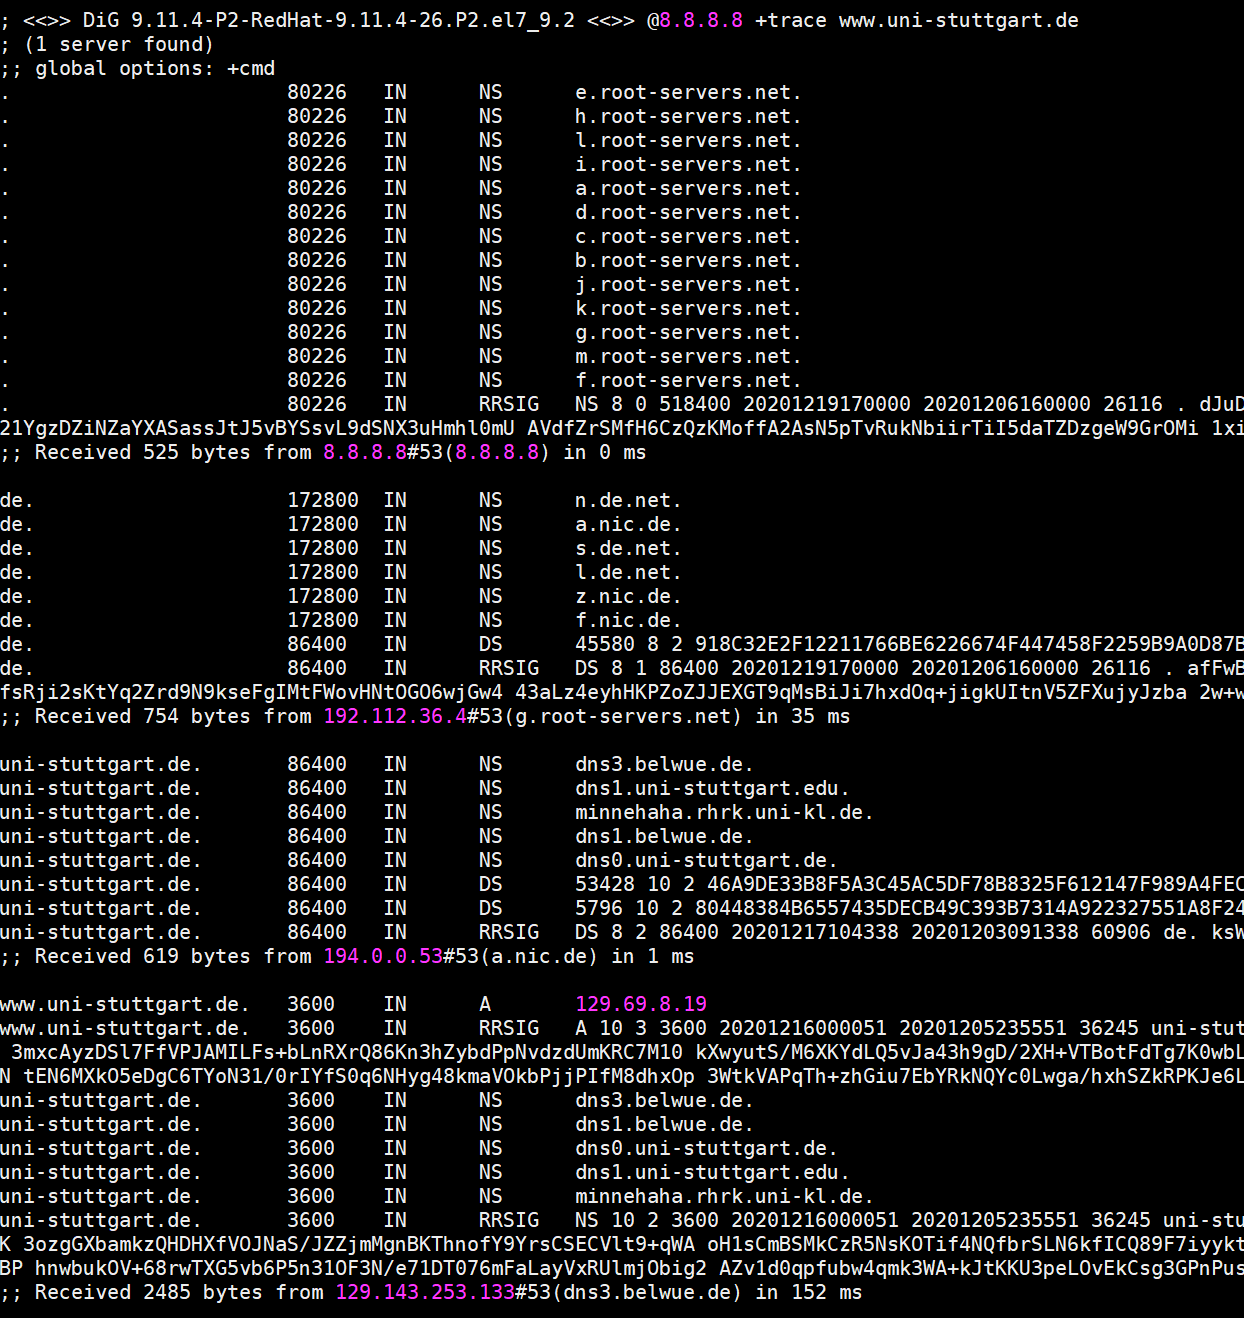
\includegraphics[scale=0.5]{dns.png}
\end{figure}
\end{document}
